\documentclass[10pt,conference]{ieeeconf}
\usepackage{amsmath}
\IEEEoverridecommandlockouts
\overrideIEEEmargins
\usepackage{cite}

%% \let\labelindent\relax
%% \usepackage{enumitem}
%% %% \setitemize{leftmargin=-12pt}
%% %% \setitemize{itemindent=-2pt}
%% \setitemize{align=left, leftmargin=6pt, labelindent=4pt, listparindent=4pt, labelwidth=3pt, itemindent=3pt}

\usepackage{graphicx}
\usepackage{afterpage}

%%\usepackage[font=small,labelfont=bf]{caption}
\usepackage[font=small,labelfont=bf,textfont=bf]{caption}




%%\setlength{\skip\footins}{0.05in}
\renewcommand{\baselinestretch}{1.0}
\newcommand{\diag}{\mbox{diag}}
\setlength{\footskip}{0pt}
\setlength{\skip\footins}{0.04in}
\makeatletter
\def\normalsize{\@setfontsize{\normalsize}{10.2bp}{10.2pt}}
\def\small{\@setfontsize{\small}{8.9bp}{9.8pt}}
\normalsize
\makeatother




\newcommand{\eqdef}{\buildrel \triangle \over =}

\begin{document}

\title{\LARGE\bf Humanoid Robot Navigation and Obstacle Avoidance \\ in
Unknown Environments \\[-0.1ex]}
\author{G. Brooks, P. Krishnamurthy, and F. Khorrami%
\thanks{The authors are with the Control/Robotics Research Laboratory
  (CRRL), Dept. of ECE,
Polytechnic Institute of NYU, Brooklyn, NY, USA.  Corresponding author: F. Khorrami, khorrami@smart.poly.edu.}}

  \maketitle
\thispagestyle{empty}
\pagestyle{empty}




\begin{abstract}
In this paper, the problem of humanoid robot navigation in an unknown environment is considered. A path planning and obstacle avoidance system based on the GODZILA algorithm is proposed. The proposed approach is computationally very light-weight and does not require building of an environment map. The algorithm follows a purely local approach based on measurements from a pair of ultrasonic sensors (sonars) mounted on the robot. A primary challenge in the implementation of the path planning and obstacle avoidance system is the limited spatial information that is available due to the wide beam angle of the sensors. However, it is seen in simulation and experimental studies in this paper that a light-weight path planning and obstacle avoidance can be implemented with these ultrasonic sensors. Also, it is shown that the spatial uncertainty inherent in these sensors can be addressed through introduction of virtual sensors based on the beam angle; this concept of virtual sensors fits nicely within the GODZILA framework that is formulated based on range measurements from an arbitrary set of sensing directions, which in this implementation, is comprised of actual sensor directions and the virtual sensor directions. The performance of the proposed algorithm is demonstrated through simulations and experimental studies utilizing a NAO humanoid robot.
\end{abstract}




    \vspace*{-0.1in}
\section{Introduction} 
    \vspace*{-0.03in}
Biped humanoid robots have attracted significant research interest over
several years along multiple research directions including sensing and
perception, obstacle detection, navigation and path planning, gait generation,
dynamic stability, and real-time control. In particular, 
navigation through an unknown environment using sensors such as vision and a
laser scanner have been addressed in many studies, e.g.,
\cite{CTS09,YKT11,MCK06,OTK05}. Walking over
uneven terrain has also been studied in \cite{IT10,CKN03,WP10}. Strategies for
stepping over obstacles have also been addressed \cite{VSY06}. Biped walking over
ramps has been addressed in \cite{LAH12} and climbing of spiral staircases has
also been studied in \cite{OGH11}. Dynamic stability of biped motion over
different types of terrain/obstacles has been addressed in \cite{WGC07,CDG08}.

In general, the problems of path planning and obstacle avoidance are relevant
in a variety of applications including unmanned vehicles and robotic arms.
Hence, path planning and obstacle avoidance algorithms 
in a variety of contexts and based on various
assumptions on environment knowledge, sensor formulations, etc.,
have been widely
studied and various approaches such as 
bug/wall-following, potential fields, graph search based methods, and
randomized algorithms 
have been addressed in the literature (e.g.,
\cite{Lat91,HA92,RN09,HNR68,Lum88,NMU99,Kha85,RK92,Ste94,KSLO96,KK05b_jirs}
and references therein). One approach specifically designed to be
computationally light-weight so as to address tight memory and processing
contraints on small autonomous vehicles is the GODZILA algorithm
\cite{KK05b_jirs}. GODZILA (Game-Theoretic Optimal
Deformable Zone with Inertia and Local Approach) is an algorithm for path
planning and obstacle avoidance for mobile robots and unmanned vehicles which provides a
solution to the navigation problem in completely unknown environments
without requiring the building of an obstacle map. GODZILA has been applied to
various types of autonomous vehicles \cite{KKN08,KK09,KK11} and can also be
used as a low-latency inner-loop obstacle avoidance within a hierarchical
structure \cite{KKN08,KK09,KK11} that combines a wide-area graph search based path planning
algorithm and a local-area
GODZILA based planner as well as optionally an intermediate-area maneuver based planner. The GODZILA algorithm utilizes a
purely local approach that minimizes memory and computational requirements.   
The desired motion direction is generated through the online minimization of an optimization cost
that incorporates three terms which penalize, respectively, motion
in directions other than the direction to the target, motion towards
obstacles, and back-tracking.  In addition to the optimization
algorithm, GODZILA includes two components:
a local straight-line planner utilized if the target is visible
and  navigation towards a random target.  To address possible local minima or
``traps'' that might occur since the algorithm follows
a local approach, a randomized component is also included in GODZILA.
When a local minimum or a ``trap'' is detected, navigation towards a
random target is initiated to escape the trap.  It was shown in \cite{KK05b_jirs} that
GODZILA provides convergence to the target in finite time with
probability 1 in any finite-dimensional space (e.g., two-dimensional and
three-dimensional environments).  GODZILA is designed to
be particularly efficient as a lightweight path planning and obstacle
avoidance algorithm suitable for small autonomous vehicles in
``urban''-like or ``office''-like environments (i.e., featuring multiple obstacles, but
with a simple topology, unlike ``maze''-like environments) capable of
operating with a small number of range sensors.


\begin{figure}[htb]
    \vspace*{-0.1in}
	\centerline{\includegraphics[width=2.6in]{nao.jpg}} 
        \caption{Aldebaran Robotics NAO humanoid robot \cite{NAO} at
      Control/Robotics Research Laboratory (CRRL).}
    \label{fig:nao}
    \vspace*{-0.1in}
\end{figure}



 
In this paper, the application of the GODZILA algorithm to humanoid robots
navigating in unknown environments is addressed utilizing ultrasonic sensors
(sonars).
While ultrasonic sensors are relatively inexpensive and compact, the spatial
obstacle information that is obtained from these sensors is relatively
low-resolution in multiple senses: a wide sonar beam within which there is no
angular information as to where the sensed return is from, low range
measurement accuracy (typically a few cm), and relatively small range (typically
a few meters). These aspects of ultrasonic sensors and methods to address
these challenges within the framework of the GODZILA algorithm are described
in Sections~\ref{nao_sec} and \ref{oas_sec}. The specific humanoid robot
platform considered in this paper is the NAO robot \cite{NAO} 
(Figure~\ref{fig:nao}) from Aldebaran Robotics. The NAO includes two
ultrasonic sensors in its standard configuration \cite{NAO_system}.


This paper is organized as follows.  The NAO robot platform and the ultrasonic sensors utilized for environment sensing are
described in Section~\ref{nao_sec}.  The GODZILA path planning and obstacle
avoidance algorithm and its application to humanoid navigation in an unknown
environment are described in Section~\ref{oas_sec}. Simulation and
experimental results are presented in Section~\ref{sim_exp_sec}.   


    \vspace*{0.02in}
\section{NAO humanoid robot and ultrasonic sensors for navigation in an unknown environment}
\label{nao_sec}
    \vspace*{0.02in}
The path planning and obstacle avoidance system proposed in this paper is
applied to the NAO (Figure~\ref{fig:nao}), a humanoid experimental platform
developed and commercialized by Aldebaran Robotics. The NAO at the
Control/Robotics Research Laboratory is a 25 degree-of-freedom humanoid
including a number of sensors (three-axis accelerometers, two one-axis gyros,
two ultrasonic sensors, four microphones, a pair of HD cameras, eight force
sensors on the bottom of the feet, and two bumpers) \cite{NAO_system}.  NAO is about 58cm tall and includes a programming framework called NAOqi that provides a user friendly interface to monitor the sensors on the NAO and send control commands to achieve higher-level robot behavior. 

The overall objective is to attain an autonomous navigation and
obstacle avoidance system for NAO utilizing the two cameras, the ultrasonic sensors onboard the robot, and possibly additional sensors. In this paper,
we are only considering the two ultrasonic sensors (Figure~\ref{fig:nao_sonar}) mounted in NAO's chest
(transmitters oriented 40 degrees apart; receivers 50 degrees apart) to show
the efficacy of our algorithm. 

The ultrasonic sensors on the NAO
robot have a resolution of 1 cm and a sensing range between 0.25 m to 2.55 m
(i.e., an obstacle which is less 0.25 m away results in a sensor measurement
of 0.25 m). 
Utilization of only the two ultrasonic sensors for environment sensing
makes the problem challenging since the ultrasonic sensors have a large
viewing cone (about 60 degrees; Figure~\ref{fig:nao_sonar}; there are also
angular and position offsets relative to the center of the robot as seen in Figure~\ref{fig:nao_sonar}) and provide one distance measurement (Figure~\ref{fig:nao_sonar_data}) from 
any obstacles within the large cone. Therefore, there will be a high degree of
uncertainty about the obstacles' location. In addition, as seen in Figure~\ref{fig:nao_sonar_data}, noisy/intermittent data is typically obtained when the sonar beams impinge on obstacles at larger oblique angles; also, spurious large values are often obtained when in close proximity to obstacles (i.e., close to the lower threshold, 25 cm, of the ultrasonic sensors). 
However, it is seen in simulation and experimental studies 
that obstacle avoidance in typical office-like environments can be implemented with these ultrasonic sensors.
In future papers, we will also consider fusing additional sensors with the ultrasonic sensors to create a robust path planning, navigation, and obstacle avoidance system.

% \begin{figure*}[htb]
% 	\centerline{\includegraphics[width=5.5in]{nao2.png}} 
%     \caption{Components of the NAO humanoid robot from Aldebaran Robotics
%     (http://www.aldebaran-robotics.com/documentation/family/nao\_h25/index\_h25.html).}
%     \label{fig:nao_arch}
% 	\hrule
% \end{figure*}

\begin{figure}[htb]
    \vspace*{-0.15in}
  \centerline{\includegraphics[width=2in,trim=0.0in 0.0in 0in 0.1in,clip=true]{sonar_diag.png}} 
        \caption{The cones corresponding to the beams for the two ultrasonic
        sensors mounted on the NAO robot.}
    \label{fig:nao_sonar}
    \vspace*{-0.2in}
\end{figure}

\begin{figure}[!h]
    \vspace*{-0.14in}
  \centerline{\includegraphics[width=3in,trim=0.0in 0.0in 0in 0.1in,clip=true]{sonar_data1.png}} 
  \caption{Typical data from NAO's ultrasonic sensors while walking down a corridor. When the wide angle sonar beams hit the walls at larger oblique angles, the acoustic returns are intermittently obtained and also contain significant multipath components. Hence, the single scalar distances obtained for each sonar show intermittent spikes between values corresponding to distance to wall, multipath distances, and maximum values (2.55 m for the NAO's ultrasonic sensors).}
    \label{fig:nao_sonar_data}
    \vspace*{-0.12in}
\end{figure}




    \vspace*{-0.03in}
\section{Application of the GODZILA algorithm to humanoid path planning and obstacle avoidance}
\label{oas_sec}
    \vspace*{-0.03in}

GODZILA \cite{KK05b_jirs} is a general computationally lightweight path planning and obstacle
avoidance algorithm that does not require any a priori knowledge of
environment and does not rely on building of an obstacle map.
GODZILA is based on three components:		
\begin{itemize}
\item
Optimization based on a cost that penalizes motion in directions other than the direction to the target, motion towards obstacles, and back-tracking.
\item
A local straight-line planner utilized if the target is visible.
\item
Navigation towards a random target when a local ``trap'' is detected.
\end{itemize}
    The desired motion direction is generated through online minimization of an optimization cost
at each sampling instant.  It can be shown that the optimization cost can
be chosen so that the minimizer can be obtained in closed form.  The
optimization cost has three terms which penalize, respectively, motion
in directions other than the direction to the target, motion towards
obstacles, and back-tracking.  In addition to the optimization
algorithm, GODZILA includes two components,
a local straight-line planner utilized if the target is visible
and  navigation towards a random target (utilized when local minima or traps
are detected). 

GODZILA can utilize obstacle range measurement data  measured using a variety of sensors such as
ultrasonic sensors or laser range finders or obstacle ranges estimated using
sensors such as camera, Radar, etc. The GODZILA algorithm is formulated in terms of a set of directions in which
obstacle range measurements are measured/estimated. Denoting by $q_i$, the
unit vector defining the $i^{th}$ sensor direction, the obstacle range
measurements/estimates are denoted as $s_i,i=1,\ldots,n$;
$s=(s_1,s_2,\ldots,s_n)$.
$x_p$ and $x_h$ are used to denote the current position and the unit vector
along the current heading, respectively, and
$u_e$ is used to denote the obstacle set (possibly time-varying) of the
environment, i.e., the set of points in the environment occupied by
obstacles. The sensors in the GODZILA algorithm are defined as returning the distance from the current position
to the obstacle set in the directions of the sensors. 
The sensor
measurements can be modified to enforce a clearance zone by
exaggerating the physical dimensions of the robot.  Since this
exaggeration is only relevant when the obstacles are close to the robot,
introducing, for instance,  
$s_i'=s_i-p_i e^{-a s_i}$
with $p_i,i=1,\ldots,n$, and $a$ being positive constants, we have
$s_i'\approx s_i$
in the far zone and 
$s_i'\approx s_i-p_i$
  in the near zone.   This weighting induces large
penalties when obstacles are near and small penalties when obstacles
are distant.  

The path planning objective is essentially to generate a trajectory that tracks a
target trajectory $x_d (t)$ (nominally a goal location $x_d$) while avoiding the obstacle set $u_e(t)$.    
The GODZILA path planning and obstacle avoidance algorithm \cite{KK05b_jirs} achieves
this objective using a combination of an optimization procedure, a
random walk, and approach to a visible target.  At any time,
the optimal heading is computed by an optimization procedure using as
effective target one of the following
\begin{enumerate}
\item The actual target $x_d$
\item A fictitious target location on an intermediate straight-line
  trajectory to the target $x_d$
\item A random target. 
\end{enumerate}
The optimization to find a desired motion direction is performed with respect to an objective function given by
$J(y)=J_1(y)+J_2(y)+J_3(y)$
which has the following three components:
\begin{enumerate}
\item $J_1(y)$ - a component that penalizes motion in directions other than the target direction, 
\item $J_2(y)$ - a component that penalizes motion towards obstacles, and
\item $J_3(y)$ - a component that penalizes back-tracking.
\end{enumerate}
The first component $J_1(y)$ attempts to make the robot move
in the direction of the target and is designed such that it is an increasing
function in terms of $\left|\left|
y-\frac{(x_d-x_p)}{||x_d-x_p||}\right|\right|$ and is a decreasing function in
terms of 
$||x_d-x_p||$
and such that in the immediate
    vicinity of the target, $J_1(y)$ is dominant in the objective function
    $J(y)$.
The second component $J_2(y)$ attempts to prevent motion in directions
that would bring the robot to the proximity of obstacles. Direction-weighted
terms \cite{KK05b_jirs} are usually included in $J_2(y)$ to model the property that the
effect of this component is more important in directions that are
either along the current heading or along the straight-line heading to
the target.   This component is designed to also encourage motion in
directions along which obstacles are far away, especially if such a
direction is along the straight-line heading to the target, and also such that in the close vicinity of obstacles, the
effect $J_2(y)$ of obstacles predominates in the objective function.
The third component $J_3(y)$ is designed to be an increasing function in terms of
$||y-x_h||$, thus penalizing
changes in heading and is
inspired by the physical notion of inertia. $J_3(y)$ is instrumental in
    preventing limit-cycle oscillations (wherein, without $J_3(y)$, oscillatory motions can arise with the obstacle avoidance incentive and the target-reaching incentive alternatively becoming dominant).  $J_3(y)$
    essentially makes a potential limit cycle spatially larger and
    hence provides better chance of finding a way around a blocking obstacle.  
If the objective function $J(y)$ has a unique minimum over the unit ball ${\cal B}=\{y:||y||=1\}$,
 the output of the algorithm
is the unique minimizer.  If the minimizer is not unique, the output
is defined as one which gives the smallest $J_3(y)$.   

It was shown in \cite{KK05b_jirs} that the 
minimizer (i.e., the optimal heading) of the objective function $J(y)$ can be
found in closed form if quadratic forms of functions are utilized within
components appearing in $J_1(y)$, $J_2(y)$, and $J_3(y)$, in which case the
 closed form optimal solution can also be equivalently interpreted in terms of force components towards
 the goal, away from obstacles, and in the current motion direction (i.e., the
 inertia component).
The desired heading found from the optimization algorithm is translated into a heading rate
that takes into account the kinematic capabilities of the robot.  
Also, 
the linear velocity of the robot is designed to be such that it is small in the close
vicinity of obstacles and in the proximity of the target location.  

As mentioned before, GODZILA also incorporates two additional components in
addition to the optimization-based computation of the optimal heading, i.e.,
a local straight-line planner utilized if the target is visible
and  navigation towards a random target.
At any time, if the target is visible, i.e., the nearest obstacle in
the direction of the target is estimated to be farther than the target, then the
robot can proceed in a straight-line towards the target.  
However, since a
direct straight-line path to the target may bring the robot in close proximity
with obstacles, the straight-line path
to the target is instead prescribed as a desired trajectory and the navigation along this path
is performed using the optimization-based approach described above. This local
straight-line based virtual reference trajectory is of particular use when
the robot needs to pass through a narrow corridor to approach the target.
The random target component addresses possible limit cycle oscillations. While the introduction of the inertial term in the
optimization cost has the effect of increasing the spatial extent of
possible limit cycles, limit cycle oscillations can still occur if the obstacle set is spatially
large since the GODZILA algorithm is
based on local sensor data and no map of the environment is built.
A local limit cycle or a {\em trap} can be detected using, for
instance, the variance of the position variable over some number of
successive sampling instants.  Alternatively, the distance to the
target can be used as a metric and a trap situation can be inferred if
this distance does not change significantly over some period of time.
If a trap is detected at a time $t_0$, a random target location $\hat x_d$ is
chosen and the navigation is performed for a time duration $T_{roam}$ using the optimization procedure
described above with $x_d$ replaced by $\hat x_d$.  
If a trap situation is detected multiple times, then progressively longer
sequences of
random moves are utilized to escape the local minima.

{\bf Virtual sensors for implementation with wide beam ultrasonic sensors:} In the application to the humanoid robot navigation problem using ultrasonic
sensors considered here, a primary sensory challenge is, as described earlier,
the wide beam angle which 
results in large angular uncertainty as to where the sonar returns are from
(i.e., the $X$-$Y$ locations of the points in the environment that correspond to
a single measured distance from each of the ultrasonic sensors). To address
this angular uncertainty, the obstacle range measurements/estimates for the
GODZILA algorithm are generated as a combination of actual and virtual sensor
measurements as follows:\\
a)
    For each ultrasonic sensor with a beam width of $\theta_w$ (which is
    60$^o$ for the ultrasonic sensors on the NAO robot), if the corresponding
    distance measurement at a sampling time is $d$, this distance measurement
    is mapped to multiple sensing directions spanning the beam width
    (typically, 5 directions, i.e., angular offsets of $0$, $\pm k
    \theta_w/2$, $k=1,2$,
    relative to the center of the sensor beam). The distance
    corresponding to the center of the sensor field of view (i.e., offset of
    $0$ degrees) is defined to be $d$ and the distances corresponding to the
    other {\em virtual} sensor directions are defined to be larger, e.g.,
    $(1+ak)d$, $k=1,2$, with $a$ being a positive constant to model the
    decreasing confidence that the returned distance values are due to
    obstacles at the edges of the beam. 
    \\
    b) The sensor measurements from a few prior sampling instants are also
    utilized as virtual sensor measurements for the current time instant. The
    robot-relative obstacle locations corresponding to the multiple virtual sensor directions
    as described above that are modeled for each ultrasonic sensor are
    utilized along with estimates of the robot pose (position and heading)
   at the previous time steps. These obstacle locations are mapped into the
   current robot-relative frame at the current time instant by utilizing
   estimates of relative translations and rotations over successive sampling
   instants. The directions corresponding to these obstacle locations are also
   now utilized as virtual sensor directions with the corresponding estimated
   ranges for the GODZILA algorithm; hence,
    the range measurements for use in the GODZILA algorithm is comprised of
    measurements over
    a sliding window of time including the current and a few past sampling
    instants. Denoting the time horizon utilized by $n_h$ and using 5 virtual sensor
    directions per sonar to model the beam width as described above, the total number of virtual
    range sensors (taking into account both the ultrasonic sensors) utilized
    in the GODZILA algorithm is $2(5)n_h=10n_h$. To model the reduction in
    confidence on the measurements from prior sampling times projected into
    the current robot pose, the weights for sensor directions corresponding to
    older time instants can be defined to be smaller in the optimization
    component $J_2(y)$ utilized in the GODZILA algorithm to penalize motion
    towards obstacles.




\noindent{\bf Remark 1:} 
More general variants of these concepts of virtual sensors are currently being
addressed in ongoing work including the incorporation of additional weighting terms on
virtual sensor directions that are more often perceived as having closer
obstacles. While implementation of the virtual sensors as described above requires keeping a
memory of a sliding window of time of sensor measurements and relative robot
poses, the resulting computational requirements (both memory and processing
requirements) are significantly lower than for incrementally building an
environment map during robot operation.  Thus, the approach proposed here provides a
computationally light-weight technique that can be easily implemented on small
embedded platforms.

\begin{figure*}[htb]
  %\centerline{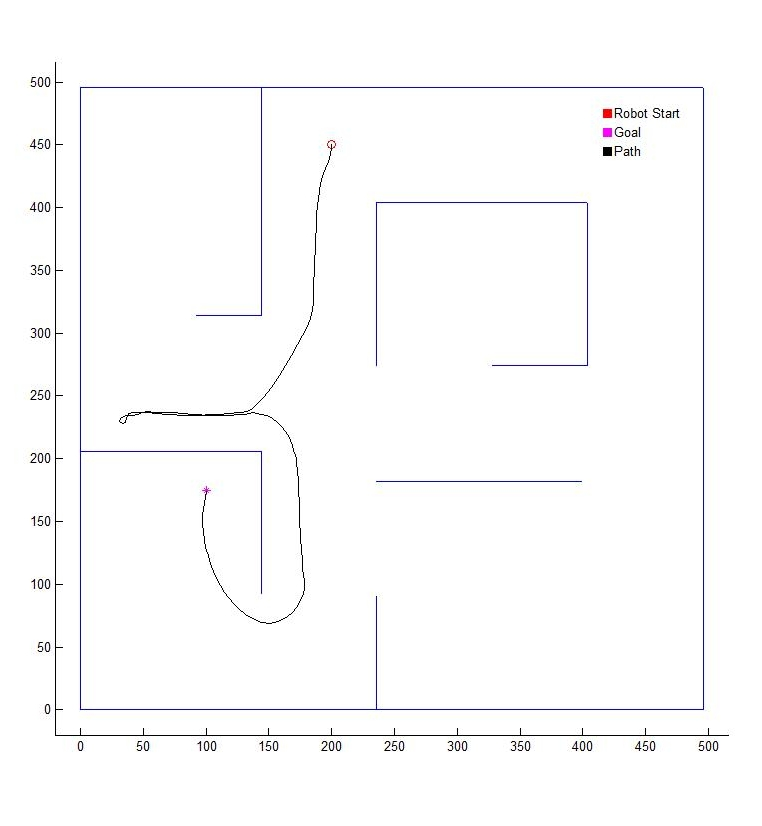
\includegraphics[width=3.2in,trim=4.0in 0.6in 2in 0.8in,clip=true]{path1.png}
  %      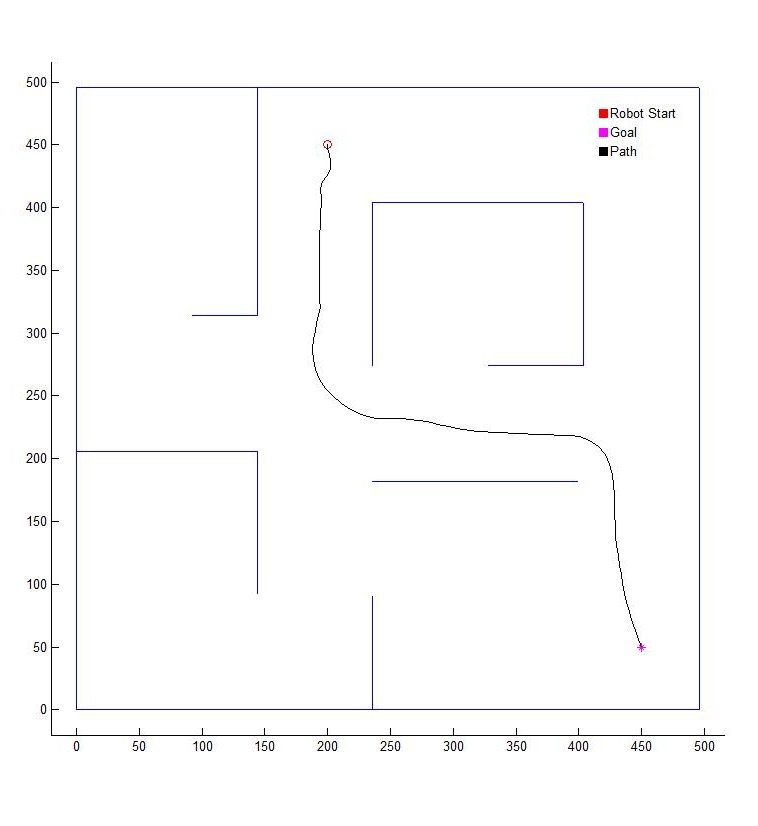
\includegraphics[width=3.2in,trim=4.0in 0.6in 2in 0.8in,clip=true]{path2.png}} 
  %      \centerline{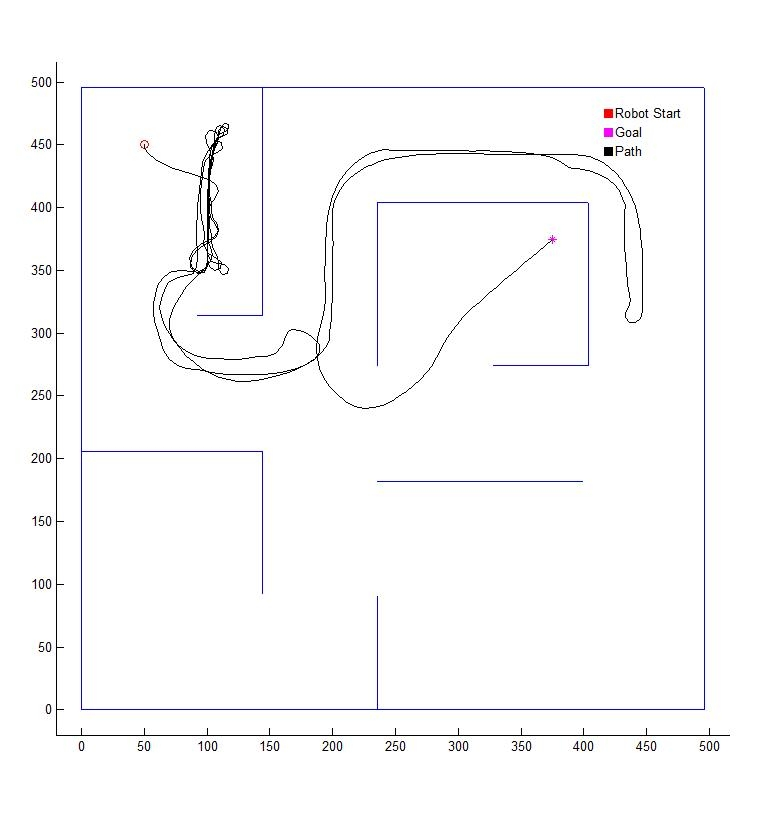
\includegraphics[width=3.2in,trim=4.0in 0.6in 2in 0.8in,clip=true]{path5.png}
  %      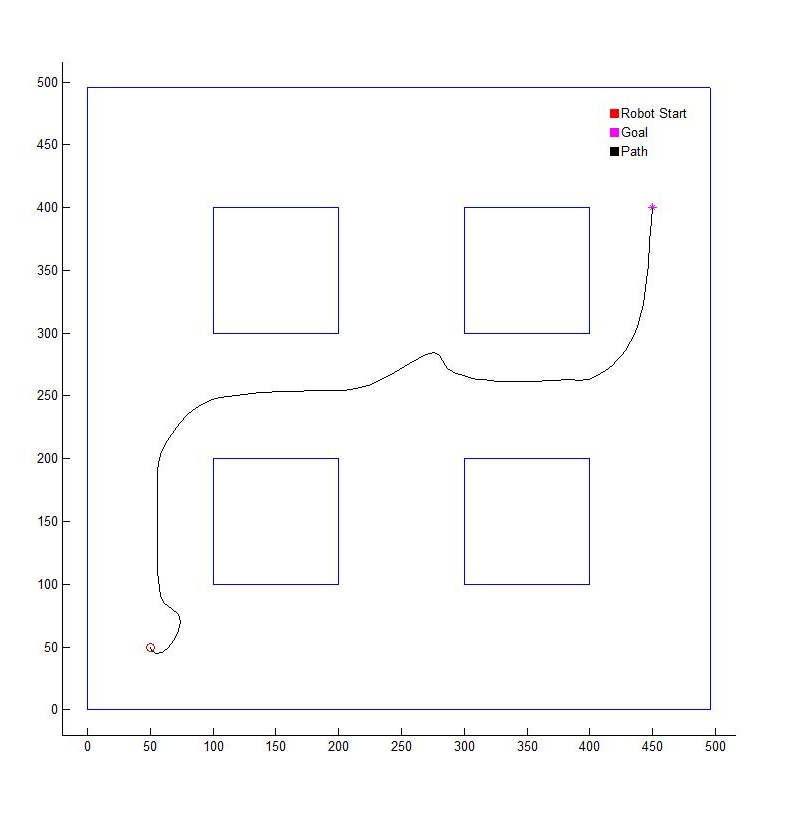
\includegraphics[width=3.2in,trim=4.0in 0.6in 2in 0.8in,clip=true]{path4.png}} 
          \centerline{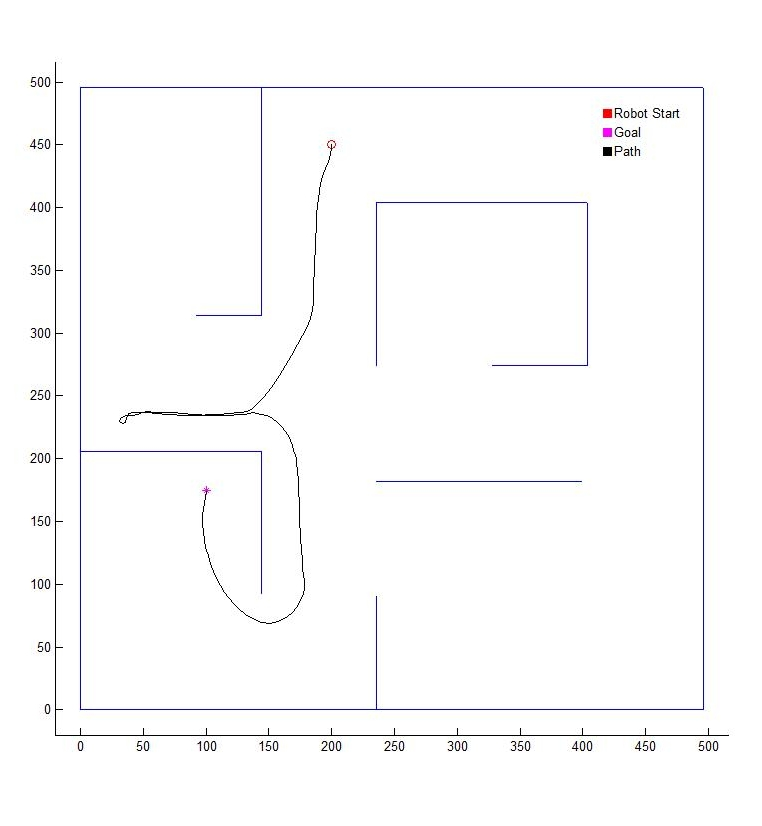
\includegraphics[width=2.8in,trim=0.2in 0.2in 0.2in 0.2in,clip=true]{path1.png}
        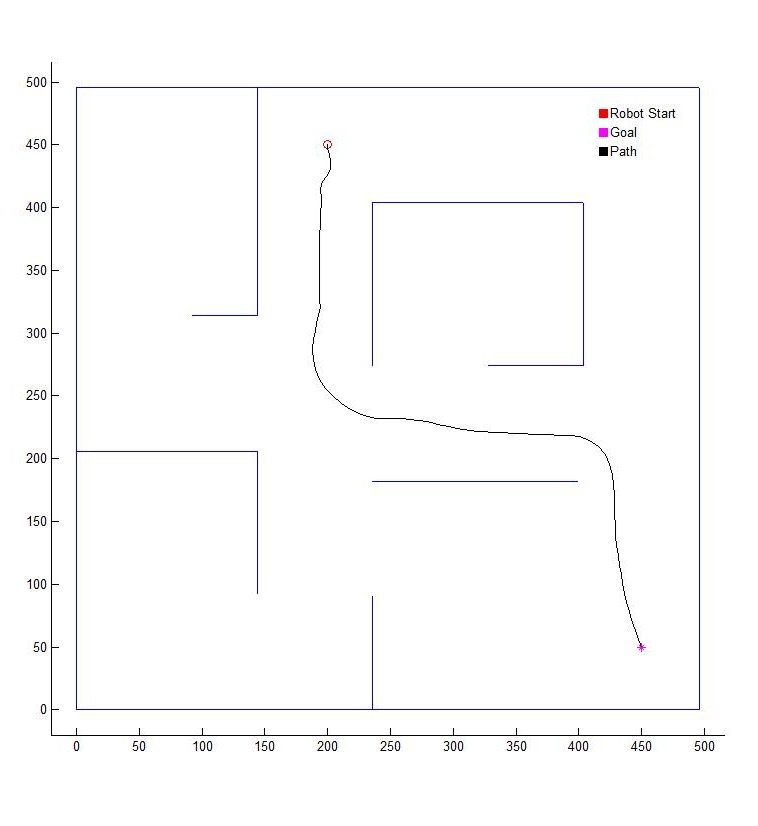
\includegraphics[width=2.8in,trim=0.2in 0.2in 0.2in 0.2in,clip=true]{path2.png}} 
	\centerline{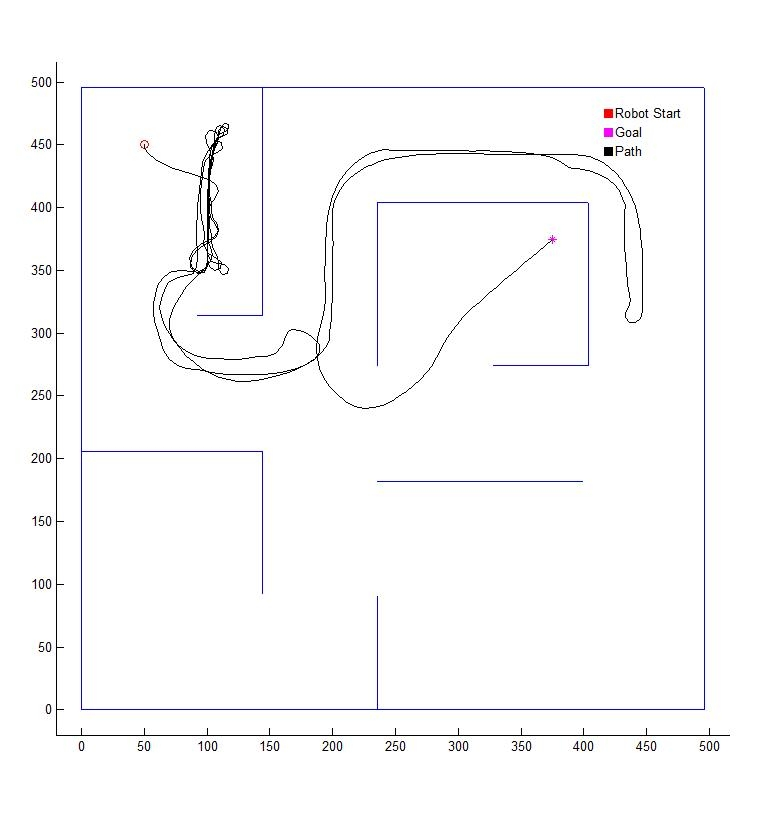
\includegraphics[width=2.8in,trim=0.2in 0.2in 0.2in 0.2in,clip=true]{path5.png}
        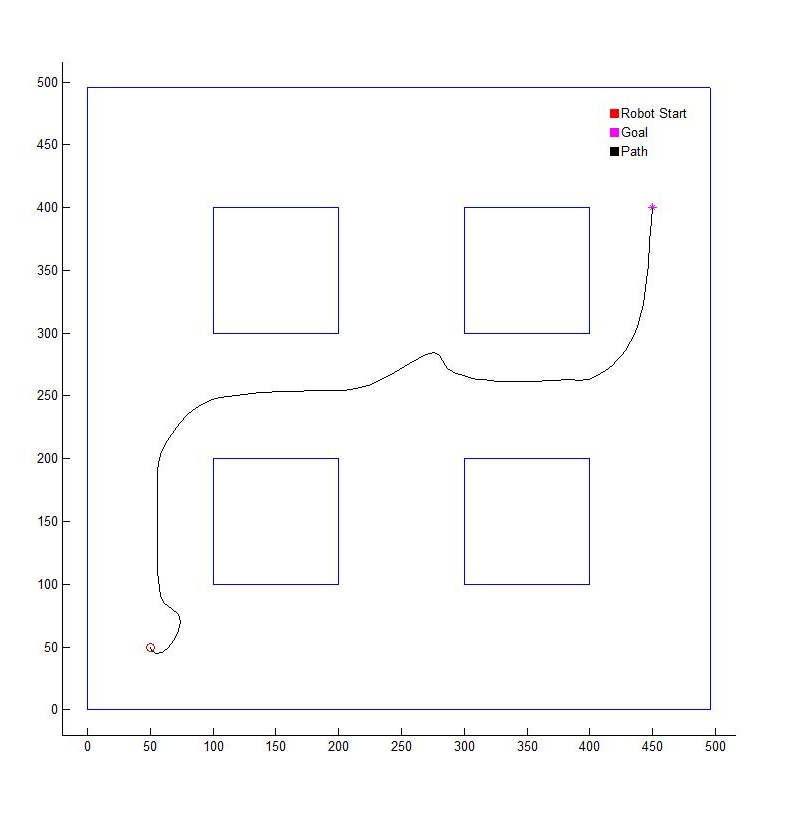
\includegraphics[width=2.8in,trim=0.2in 0.2in 0.2in 0.2in,clip=true]{path4.png}} 

    \caption{Simulation results utilizing a pair of ultrasonic sensors mounted
    on the NAO humanoid robot. In these figures, the robot start and goal
  locations are shown in red and magenta, respectively. The trajectory of the
robot is shown as a black line. The obstacles in the environment are shown as
blue lines. The $X$ and $Y$ axis dimensions in the figures are in cm. The
environment is taken to be unknown and the robot navigates utilizing the
ultrasonic sensor measurements (one measurement at each sampling instant from
each of the two ultrasonic sensors) based on the GODZILA algorithm. Due to the
large angular uncertainty inherent in the ultrasonic sensor measurements, some
amount of meandering can be sometimes seen (as in the figure on the bottom
left); however, the detection of local minima (or traps) and subsequent random
walk components built into GODZILA ensure that the robot eventually finds a
path to the goal location.}
    \label{fig:simfig1}
	\hrule
        \vspace*{-0.3in}
\end{figure*}

    \vspace*{-0.03in}
\section{Simulation and Experimental Studies}
\label{sim_exp_sec}
    \vspace*{-0.03in}
The performance of the proposed approach for humanoid path planning and
obstacle avoidance is illustrated in this section based on simulation and
experimental studies using a NAO humanoid robot (Figure~\ref{fig:nao}).
For simulation studies, a simulator for the NAO robot and the pair of
ultrasonic sensors has been implemented taking into account the sensor
geometry, beam width, resolution, and noise. Simulations in an unknown
environment and with several choices of initial and final locations are shown
in Figure~\ref{fig:simfig1}.  The robot navigates in the unknown environment
utilizing the distance measurements from the ultrasonic sensors based on the
GODZILA algorithm. In Figure~\ref{fig:simfig1}, the robot start and goal
  locations are shown in red and magenta, respectively, the trajectory of the
robot is shown as a black line, and the obstacles in the environment are shown as
blue lines. Experimental testing on the NAO robot is illustrated in
Figure~\ref{fig:nao_exp}. Two experimental runs are shown in Figure~\ref{fig:nao_exp}. 
In the experimental run shown on the left in Figure~\ref{fig:nao_exp}, the robot is positioned facing an obstacle around which it needs to
    navigate while walking down a corridor. In the experimental run shown on the right, the red marker near the far wall is prescribed as the goal location that the robot has to reach while avoiding obstacles; in this experimental run, the onboard cameras on the NAO are utilized for detection and tracking of the red marker (estimation of relative range and bearing of the goal position relative to the robot) while the obstacle avoidance utilizes only the pair of ultrasonic sensors.
It is seen that the ultrasonic sensors enable a reasonable level of obstacle avoidance in typical environments. However, as described in Section~\ref{nao_sec}, the ultrasonic sensors have a wide field of view resulting in large spatial uncertainty and can also provide spurious/noisy distance measurements in some obstacle configurations, which can result in erratic robot behavior during obstacle avoidance using only ultrasonic sensors. In on-going work, the incorporation of additional sensors for obstacle avoidance such as a set of ultrasonic
sensors with a more narrow beam as well as other sensors is also being considered.





\begin{figure*}[!th]
%  \centerline{\includegraphics[width=1.5in]{a1.jpg}
%  \includegraphics[width=1.5in]{a2.jpg}
%  \includegraphics[width=1.5in]{a3.jpg}
%} \vspace*{0.05in}
%  \centerline{\includegraphics[width=1.5in]{a4.jpg}
%  \includegraphics[width=1.5in]{a5.jpg}
%  \includegraphics[width=1.5in]{a6.jpg}
%}
%
  %\vspace*{-0.0in}
  \begin{tabular}{p{3.2in}|p{3.2in}}
  \centerline{\includegraphics[width=1.25in]{a1.jpg}
  \includegraphics[width=1.25in]{a2.jpg}
} 
\vspace*{0.05in}
\centerline{\includegraphics[width=1.25in]{a3.jpg}
\includegraphics[width=1.25in]{a4.jpg}}
\vspace*{0.05in}
 \centerline{\includegraphics[width=1.25in]{a5.jpg}
  \includegraphics[width=1.25in]{a6.jpg}}
  \vspace*{-0.2in}
  &
  \centerline{\includegraphics[width=1.25in]{exp1_1s.jpg}
  \includegraphics[width=1.25in]{exp1_2s.jpg}
} 
\vspace*{0.05in}
\centerline{\includegraphics[width=1.25in]{exp1_4s.jpg}
\includegraphics[width=1.25in]{exp1_5s.jpg}}
\vspace*{0.05in}
 \centerline{\includegraphics[width=1.25in]{exp1_6s.jpg}
  \includegraphics[width=1.25in]{exp1_7s.jpg}}
  \vspace*{-0.2in}
\end{tabular}
    \caption{Experimental results utilizing a pair of ultrasonic sensors mounted
    on the NAO humanoid robot. Pictures from two experimental runs are shown in the figure above. In each experimental run, the pictures above show the time sequence of
    robot poses (left to right in top row followed by left to right in middle
    row followed by left to right in bottom row). 
  %  Various versions of the path planning and obstacle avoidance algorithms including non-goal-directed exploration-style algorithms (wherein the robot moves around the environment randomly while avoiding obstacles) as well as simple algorithms based on differential sensor measurements are being studied on the NAO robot. In current ongoing work, tuning guidelines/algorithms for various parameters (both constant weights and functions in the optimization costs) within the GODZILA algorithm are being experimentally studied.
  }
    \label{fig:nao_exp}
	\hrule
        \vspace*{-0.27in}
\end{figure*}



    \vspace*{-0.03in}
\section{Conclusion}
    \vspace*{-0.03in}
In this paper, a computationally light-weight approach for path planning and
obstacle avoidance for humanoid robots operating in unknown environments was
proposed based on inexpensive ultrasonic sensors. The proposed algorithm does
not require any prior knowledge of the operating environment and does not rely
upon building of a map of the environment, thus minimizing the memory and
computational requirements of the algorithm. The efficacy of the proposed
approach was demonstrated through simulation and experimental studies. 
In current ongoing work, the performance of the proposed algorithm is being
further tested under various simulated and experimental obstacle environments; also, tuning guidelines/algorithms for various parameters (both constant weights and
functions in the optimization costs) within the GODZILA algorithm are being
experimentally studied.
Also, the incorporation of additional sensors such as a set of ultrasonic
sensors with a more narrow beam as well as other sensors is also being considered in ongoing work. 
In future work, the application of the proposed approach to other scenarios
such as leader following (e.g., following a human leader through an office-like
environment) will also be addressed.

      
%\afterpage{\clearpage}


\renewcommand{\baselinestretch}{0.97}
    \vspace*{-0.06in}
\begin{thebibliography}{10}
\providecommand{\url}[1]{#1}
\csname url@rmstyle\endcsname
\providecommand{\newblock}{\relax}
\providecommand{\bibinfo}[2]{#2}
\providecommand\BIBentrySTDinterwordspacing{\spaceskip=0pt\relax}
\providecommand\BIBentryALTinterwordstretchfactor{4}
\providecommand\BIBentryALTinterwordspacing{\spaceskip=\fontdimen2\font plus
\BIBentryALTinterwordstretchfactor\fontdimen3\font minus
  \fontdimen4\font\relax}
\providecommand\BIBforeignlanguage[2]{{%
\expandafter\ifx\csname l@#1\endcsname\relax
\typeout{** WARNING: IEEEtran.bst: No hyphenation pattern has been}%
\typeout{** loaded for the language `#1'. Using the pattern for}%
\typeout{** the default language instead.}%
\else
\language=\csname l@#1\endcsname
\fi
#2}}

\bibitem{CTS09}
J.~Chestnutt, Y.~Takaoka, K.~Suga, K.~Nishiwaki, J.~Kuffner, and S.~Kagami,
``Biped navigation in rough environments using on-board sensing,'' in
\emph{Proc. of the IEEE/RSJ International Conf. on Intelligent
Robots and Systems}, (St. Louis, MO), Oct. 2009.

\bibitem{YKT11}
A.~Yamashita, M.~Kitaoka, and T.~Kaneko, ``Motion planning of biped robot
equipped with stereo camera using grid map,'' \emph{International Jour. of
Automation Technology}, vol.~5, no.~5, pp.~639-647, 2011.

\bibitem{MCK06}
P.~Michel, J.~Chestnutt, S.~Kagami, K.~Nishiwaki, J.~Kuffner, and T.~Kanade,
``Online environment reconstruction for biped navigation,'' in
\emph{Proc. of the IEEE International Conf. on Robotics and
Automation}, (Orlando, Florida), May 2006.

\bibitem{OTK05}
R. Ozawa, Y. Takaoka, Y. Kida, K. Nishiwaki, J. Chestnutt, J. Kuffner, S.
Kagami, H. Mizoguch, and H. Inoue, ``Using visual odometry to create 3D maps
for online footstep planning,'' in \emph{Proc. of the IEEE International
Conf. on Systems, Man and Cybernetics}, (Big Island, HI), Oct. 2005.

\bibitem{IT10}
F. Iida and R. Tedrake, ``Minimalistic control of biped walking in rough
terrain,'' \emph{Autonomous Robots}, pp. 355-368, April 2010.

\bibitem{CKN03}
J. Chestnutt, J. Kuffner, K. Nishiwaki, and S. Kagami, ``Planning biped
navigation strategies in complex environments,'' in \emph{Proc. of the
2003 IEEE International Conf. on Humanoid Robotics}, (Karlsruhe, Germany), Sept. 2003.

\bibitem{WP10}
J.-c. Wu and Z. Popovi\'c, ``Terrain-adaptive bipedal locomotion control,''
\emph{ACM Trans. on Graphics}, vol. 29, no. 4, July 2010.

\bibitem{VSY06}
B. Verrelst, O. Stasse, K. Yokoi, B. Vanderborght, ``Dynamically stepping over
obstacles by the humanoid robot HRP-2,'' in \emph{Proc. of the IEEE-RAS
International Conf. on Humanoid Robots}, (Genova, Italy), Dec. 2006.

\bibitem{LAH12}
C. Lutz, F. Atmanspacher, A. Hornung, and M. Bennewitz, ``NAO walking down a
ramp autonomously,'' in \emph{Proc. of the IEEE/RSJ International
Conf. on Intelligent Robots and Systems}, (Vilamoura, Portugal), Oct. 2012.

\bibitem{OGH11}
S. Oswald, A. Gorog, A. Hornung, and M. Bennewitz, ``Autonomous climbing of
spiral staircases with humanoids,'' in \emph{Proc. of the IEEE/RSJ
International Conf. on Intelligent Robots and Systems}, (San Francisco, CA), Sept. 2011.

\bibitem{WGC07}
E.R. Westervelt, J.W. Grizzle, C. Chevallereau, J.H. Choi, and B. Morris.  Feedback
control of dynamic bipedal robt locomotion. \emph{CRC Press}, 2007.

\bibitem{CDG08}
C. Chevallereau, D. Djoudi, and J.W. Grizzle, ``Stable bipedal walking with
foot rotation through direct regulation of the zero moment point'', \emph{IEEE
Trans. on Robotics}, vol. 25, no. 2, pp.~390-401, April 2008.



\bibitem{Lat91}
J.~C. Latombe, \emph{Robot Motion Planning}.\hskip 1em plus 0.5em minus
  0.4em\relax Norwell, MA: Kluwer Academic Publishers, 1991.

\bibitem{HA92}
Y.~K. Hwang and N.~Ahuja, ``Gross motion planning - a survey,'' \emph{ACM
  Computing Surveys}, vol.~24, no.~3, pp. 219--291, Sep. 1992.

\bibitem{RN09}
S.~Russell and P.~Norvig, \emph{Artificial Intelligence: A Modern Approach}. Saddle River, NJ: Prentice Hall, 2009.


  \bibitem{HNR68}
P.~E. Hart, N.~J. Nilsson, and B.~Raphael,
``A formal basis for the heuristic determination of minimum cost paths,''
\emph{IEEE Trans. on Systems Science and Cybernetics},
  vol.~SSC-4, no.~2, pp.~100--107, July 1968.  


\bibitem{Lum88}
V.~Lumelsky, ``On the connection between maze-searching and robot motion
  planning algorithms,'' in \emph{Proc. of the IEEE Conf. on
  Decision and Control}, Austin, TX, Dec. 1988, pp. 2270--2275.


\bibitem{NMU99}
H.~Noborio, Y.~Maeda, and K.~Urakawa, ``Three or more dimensional sensor-based
  path-planning algorithm {HD-I},'' in \emph{Proc. of the IEEE
  International Conf. on Intelligent Robots and Systems}, Kyongju, Korea,
  Oct. 1999, pp. 1699--1706.

\bibitem{Kha85}
O.~Khatib, ``Real-time obstacle avoidance for manipulators and mobile robots,''
  in \emph{Proc. of the IEEE International Conf. on Robotics and
  Automation}, March 1985, pp. 500--505.

\bibitem{RK92}
E.~Rimon and D.~E. Koditschek, ``Exact robot navigation using artificial
  potential functions,'' \emph{IEEE Trans. on Robotics and Automation},
  vol.~8, no.~5, pp. 501--518, Oct. 1992.


\bibitem{Ste94}
A.~Stentz, ``Optimal and efficient path planning for partially-known
  environments,'' in \emph{Proc. of the IEEE International Conf. on
  Robotics and Automation}, San Diego, CA, May 1994, pp. 3310--3317.


\bibitem{KSLO96}
L.~E. Kavraki, P.~Svestka, J.-C. Latombe, and M.~H. Overmars, ``Probabilistic
  roadmaps for path planning in high-dimensional configuration spaces,''
  \emph{IEEE Trans. on Robotics and Automation}, vol.~12, no.~4, pp.
  566--580, Aug. 1996.


\bibitem{KK05b_jirs}
P.~Krishnamurthy and F.~Khorrami, ``{GODZILA}: A low-resource algorithm for
  path planning in unknown environments,'' \emph{Jour. of Intelligent and Robotic Systems}, vol.~48, no.~3, pp.~357--373, March 2007.

  \vspace*{0.01in}
\bibitem{KKN08}
P.~Krishnamurthy, F.~Khorrami, and T.~L.~Ng, ``Obstacle avoidance for unmanned sea surface vehicles: a hierarchical approach,'' in \emph{Proc. of the 2008 IFAC World Congress}, Seoul, Korea, July 2008.

  \vspace*{0.01in}
\bibitem{KK09} 
F. Khorrami and P. Krishnamurthy, ``A hierarchical path planning and obstacle
avoidance system for an autonomous underwater vehicle,'' in \emph{Proc.
of the American Control Conf.}, (St. Louis, MO), June 2009.

  \vspace*{0.02in}
\bibitem{KK11} 
P. Krishnamurthy and F. Khorrami, ``A hierarchical control and obstacle
avoidance system for Unmanned Sea Surface Vehicles,'' in \emph{Proc. of
the IEEE Conf. on Decision and Control/ European Control Conf.},
(Orlando, FL), pp. 2070--2075, Dec. 2011.

  \vspace*{0.03in}
\bibitem{NAO}
NAO Humanoid Robot. \url{http://www.aldebaran-robotics.com}.


  \vspace*{0.03in}
\bibitem{NAO_system}
Components of NAO Humanoid Robot. \url{http://www.aldebaran-robotics.com/documentation/family/nao\_h25/index\_h25.html}.
\end{thebibliography}


\end{document}


